\documentclass[12pt]{article}
\usepackage[margin=1in]{geometry}
\usepackage{amsmath, amsthm, amssymb, amsfonts, enumitem, graphicx}

\theoremstyle{definition}
\newtheorem{problem}{Problem}
\renewcommand*{\proofname}{Solution}
\renewcommand{\theenumi}{\alph{enumi}}

\newcommand{\vect}[1]{\boldsymbol{#1}}

\title{Homework Assignment 1}
\author{Matthew Tiger}


\begin{document}


\maketitle


% Problem 1
\begin{problem}
  To be comprehensive, the second derivative test for two-variable functions $f = f(x, y)$
  studied in Calculus III should contain (among others) the cases:
  \begin{enumerate}
    \item $D(a, b) > 0$ and $f_{xx}(a, b) = 0,$
    \item $D(a, b) = 0$ and $f_{xx}(a, b) = 0.$
  \end{enumerate}
  Why aren't these cases considered? Explain.
\end{problem}

\begin{proof}
  Throughout, we assume that $f: S \subset \mathbb{R}^2 \to \mathbb{R}$ and that $f \in C^2(S)$ so
  that $f_{xy}(a,b) = f_{yx}(a,b)$. Therefore,
  \begin{align*}
    D(a, b)
    &= f_{xx}(a,b) f_{yy}(a,b) - f_{xy}(a,b)f_{yx}(a,b) \\
    &= f_{xx}(a,b) f_{yy}(a,b) - f_{xy}(a,b)^2.
  \end{align*}

  \begin{enumerate}
    \item To illustrate that this case can never happen, suppose to the contrary
      that $D(a, b) > 0$ and $f_{xx}(a, b) = 0.$ Since
      $D(a, b) = f_{xx}(a,b) f_{yy}(a,b) - f_{xy}(a,b)^2,$
      we see that $0 < D(a, b) = - f_{xy}(a,b)^2$ which is a contradiction since
      $f_{xy}(a,b)^2 > 0$. Therefore, this case cannot happen.
    \item Now suppose that $D(a, b) = 0$ and $f_{xx}(a, b) = 0$. As
      $D(a, b) = f_{xx}(a,b) f_{yy}(a,b) - f_{xy}(a,b)^2,$
      it is true under our supposition that $f_{xy}(a,b)^2 = 0$, i.e.\ $f_{xy}(a,b) = 0$.
      We cannot conclusively state whether the point is a local extrema or saddle point as the function could be increasing or decreasing in the direction of $x$ or $y$.

      To illustrate, take as an example $f_1(x, y) = -x^4 - y^4$ and $f_2(x, y) = x^4 + y^4$.
      Note that $f_1$ and $f_2$ both satisfy $D(a,b) = 0$ and $f_{xx}(a,b) = 0$ for the point $(a, b) = (0, 0)$.
      However, upon further inspection $f_1$ obtains a local maximum at $(0, 0)$, yet
      $f_2$ obtains a local minimum at $(0, 0)$. Thus, two different results occur for two different functions
      in the case where $D(a, b) = 0$ and $f_{xx}(a, b) = 0$ and we conclude that the
      test is inconclusive in such cases.

  \end{enumerate}
\end{proof}
\newpage


% Problem 2
\begin{problem}
  Recall that
  \begin{itemize}
    \item $(a, b)$ is called an \textit{absolute maximum} of $f = f(x, y)$ on a domain
      $D \subset \mathbb{R}^2$ if $f(x, y) \leq f(a, b)$
      for every $(x, y) \in D$.
    \item (The Extreme Value Theorem) If $f$ is continuous and $D$ is closed and bounded,
      then $f$ attains both an absolute maximum value and an absolute minimum value.
  \end{itemize}
  \begin{enumerate}
    \item Describe in steps (and in words) how one finds absolute extrema for a two-variable
      function $f = f(x, y)$ on a closed bounded $D \subset \mathbb{R}^2$.
    \item Apply your procedure derived in (a) to find absolute extrema for
      $f(x, y) = 2x^3 + xy^2 + 5x^2 + y^2$
      over the rectangle $D := \{(x, y)\ | -2 \leq x \leq 3, 0 \leq y \leq 2\}$.
  \end{enumerate}
\end{problem}

\begin{proof}
  \begin{enumerate}
    \item The steps below outline the process to obtain the absolute extreme for
      a two-variable, continuous function $f = f(x, y)$ on a closed bounded $D \subset \mathbb{R}^2$.
      \begin{enumerate}[label=\Roman*.]
        \item First, identify the critical points of the function, i.e. find the points
          $(x_i, y_i)$ such that $$\bigtriangledown f(x_i, y_i) = \langle f_x(x_i, y_i), f_y(x_i, y_i) \rangle = \langle 0, 0 \rangle$$
          or such that $f_x(x_i, y_i)$ or $f_y(x_i, y_i)$ do not exist.
        \item Suppose that $S_f$ is the set of critical points obtained in step I. Then
          $P = S_f \cap D$ is the set of possible points at which
          the function $f$ obtains its absolute minimum and maximum on the closed bounded domain $D$.
        \item Note that our function satisfies
          the assumptions of The Extreme Value Theorem and as a result, using the set $P$ obtained in step II,
          $\max{f(P)}$ is the absolute maximum of the function $f$
          and $\min{f(P)}$ is the absolute minimum of the function $f$.
      \end{enumerate}
    \item Let $f(x, y) = 2x^3 + xy^2 + 5x^2 + y^2$ where $f: D = \{(x, y)\ | -2 \leq x \leq 3, 0 \leq y \leq 2\} \to \mathbb{R}^2$. Then
      \begin{align*}
        \bigtriangledown f(x, y) = \langle f_x(x, y), f_y(x, y) \rangle = \langle 2x(3x + 5) + y^2, 2y(x + 1)\rangle.
      \end{align*}
      Note that $f_y(x,y) = 0$ if $x = -1$ or $y = 0$ as the real numbers form a field and thus form an integral domain.
      Also note that $f_x(x, y) = 0$ if $x = -1$ and $y = \pm 2$ or $x = -5/3$ and $y = 0$ or $x = 0$ and $y = 0$. Thus,
      $\bigtriangledown f(x, y) = \langle 0, 0 \rangle$ if $(x, y) \in \{(-5/3, 0), (-1, -2), (-1, 2), (0, 0)\} = S_f$.  Since the partial derivatives
      of $f$ exist everywhere, the set $S_f$ contains every critical point of the function $f$.

      Now, $P = S_f \cap D = \{(-5/3, 0), (-1, 2), (0, 0)\}$ and $f(P) = \{125/27, 3, 0\}$. Therefore,
      the absolute maximum of $f$ is $\max{f(P)} = 125/27$ which occurs at the point $(-5/3, 0)$ and the absolute
      minimum of $f$ is $\min{f(P)} = 0$ which occurs at the point $(0, 0)$.
  \end{enumerate}
\end{proof}
\newpage


% Problem 3
\begin{problem}
  Consider the optimization problem:
  \begin{align*}
    \begin{array} {lcl}
      \text{Min (Max) } & f(x_1, x_2, \dots, x_n) & \\
      \text{subject to } & g_1(x_1, x_2, \dots, x_n) &= k_1 \\
      & g_2(x_1, x_2, \dots, x_n) &= k_2 \\
      & \vdots & \\
      & g_m(x_1, x_2, \dots, x_n) &= k_m \\
    \end{array}
  \end{align*}
  \begin{enumerate}
    \item Formulate the Lagrangean and describe how we should proceed in order
      to solve such a problem.
    \item Find the relative extrema of $f(x, y, z) = x + 2y + 3z$ subject to
      $x - y + z = 1, x^2 + y^2 = 1$.
  \end{enumerate}
\end{problem}

\begin{proof}
  \begin{enumerate}
    \item The Lagrangean associated to the optimization problem is the equation
      \begin{align*}
        L(x_1, \dots, x_n, \lambda_1, \dots, \lambda_m) = f(x_1, \dots, x_n) + \sum_{i=1}^m \lambda_i (k_i -g_i(x_1, \dots, x_n)).
      \end{align*}
      Note that if the vector $(x_1, \dots, x_n)$ minimizes (maximizes) the objective
      function, then there exists a vector $(\lambda_1, \dots, \lambda_m)$ such that
      \begin{align}\label{gradient}
        \bigtriangledown L(x_1, \dots, x_n, \lambda_1, \dots, \lambda_m) = (0, \dots, 0, 0, \dots, 0).
      \end{align}
      Thus, in order to find the optimal value of the objective function
      we must find all vectors $(x_1, \dots, x_n, \lambda_1, \dots, \lambda_m)$
      that satisfy \eqref{gradient}. Note that the partials of $L$ with respect to $\lambda_i$ return the original
      constraints. Then from that collection of vectors, test the
      values $(x_1, \dots, x_n)$ in the objective function
      and the vector that minimizes (maximizes) the function is the optimal solution.
    \item The Lagrangean associated to this problem is given by
      \begin{align}
        L(x, y, z, \lambda_1, \lambda_2) = x + 2y + 3z + \lambda_1(1 - (x - y + z)) + \lambda_2(1 - (x^2 + y^2))
      \end{align}
      It is straightforward to compute the partials of $L$ with respect to the variables
      $x, y, z$ and these computations are presented below:
      \begin{align*}
        \begin{array}{lll}
          L_x &= 1 - \lambda_1 - 2\lambda_2 x &= 0 \\
          L_y &= 2 + \lambda_1 - 2\lambda_2 y &= 0 \\
          L_z &= 3 - \lambda_1 &= 0
        \end{array}
      \end{align*}
      From these equations we can see that the solution vector in terms of $\lambda_1$ and
      $\lambda_2$ is given by
      $$(x, y, z, \lambda_1, \lambda_2) = \left (-\frac{1}{\lambda_2}, \frac{5}{2\lambda_2}, z, 3, \lambda_2\right).$$
      Using this vector, we solve the original constraints for the possible values of $z$ and $\lambda_2$ and
      see that
      \begin{align}
        \begin{array}{lll}
          \vect{v_1} &= (x_1, y_1, z_1, \lambda_{11}, \lambda_{12}) &=\left( -\frac{2}{\sqrt{29}}, \frac{5}{\sqrt{29}}, 1 + \frac{7}{\sqrt{29}}, 3, \frac{\sqrt{29}}{2} \right)\\
          \vect{v_2} &= (x_2, y_2, z_2, \lambda_{21}, \lambda_{22}) &=  \left( \frac{2}{\sqrt{29}}, -\frac{5}{\sqrt{29}}, 1 - \frac{7}{\sqrt{29}}, 3, -\frac{\sqrt{29}}{2} \right)
        \end{array}
      \end{align}
      are the possible values of $x, y, z, \lambda_1, \lambda_2$ that satisfy \eqref{gradient}.
      Using $\vect{v_1}$ and $\vect{v_2}$ we see that
      \begin{align*}
        \begin{array}{lll}
          f(x_1, y_1, z_1) &= 3 + \sqrt{29}  &\approx 8.38516\\
          f(x_2, y_2, z_2) &= 3 - \sqrt{29} &\approx -2.38516\\
        \end{array}
      \end{align*}
      so that $3 + \sqrt{29} $ is a relative maximum at $\left( -\frac{2}{\sqrt{29}}, \frac{5}{\sqrt{29}}, 1 + \frac{7}{\sqrt{29}}\right)$ and
      $3 - \sqrt{29}$ is a relative minimum at $\left( \frac{2}{\sqrt{29}}, -\frac{5}{\sqrt{29}}, 1 - \frac{7}{\sqrt{29}}\right)$.
  \end{enumerate}
\end{proof}
\newpage


% Problem 4
\begin{problem}
  Solve the shipping problem studied in MATH 111 if we replace the constraint
  $x + 2y \leq 100$ by the constraint $x + 2y \leq 625/6$. Use Mathematica to
  (at least) graph the feasible set.
\end{problem}

\begin{proof}
  The linear program associated to the shipping problem with the replaced constraint
  is presented below:
  \begin{align*}
    \begin{array} {lll}
      \text{Maximize} & 13x + 9y & \\
      \text{subject to} & 4x + 3y &\leq 300 \\
      & x + 2y &\leq 625/6\\
      & -2x + y &\leq 0 \\ \\
      & x \geq 0, y \geq 0 & \\
    \end{array}
  \end{align*}

  The following Mathematica commands plot the feasible region of the linear
  program and find the solution to the linear program.
  \begin{figure}[!h]
    \centerline{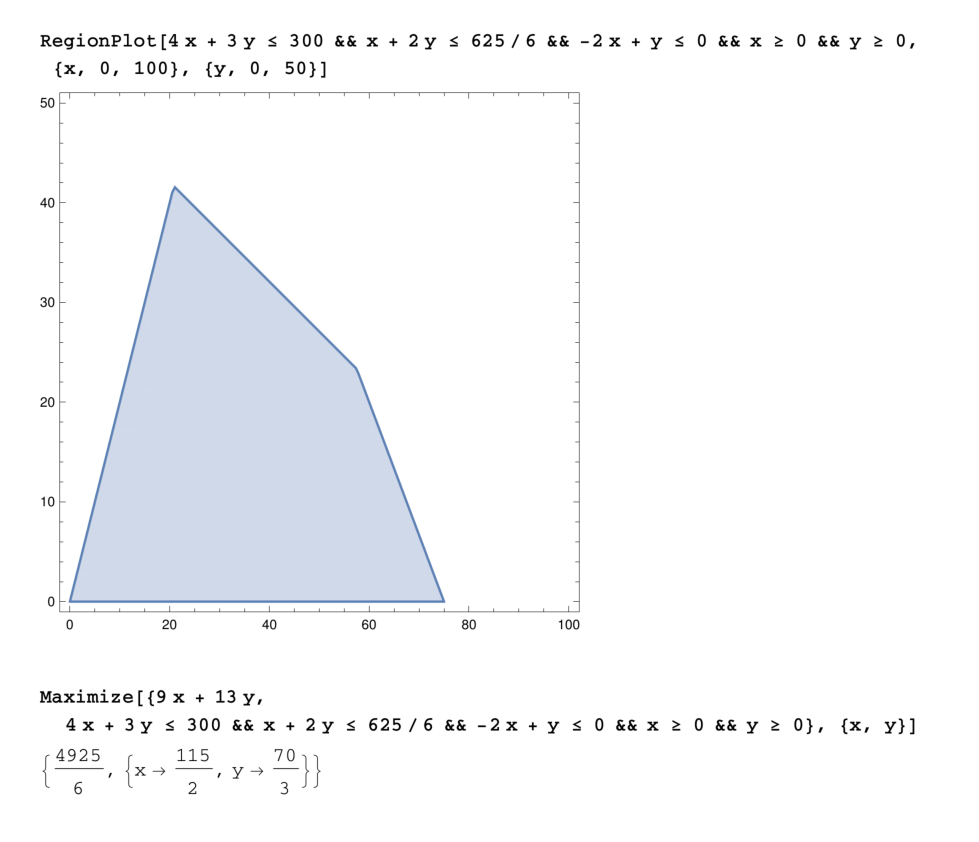
\includegraphics[scale=1.0]{linear_program}}
  \end{figure}

  As we can see, the objective function is maximized under the given constraints
  when $x = 75$ and $y = 0$ leading to an objective function value of 975.
\end{proof}
\newpage


% Problem 5
\begin{problem}
  Suppose that $f, f_1, f_2$ are convex functions and $a \geq 0$. Prove that
  $af$ and $f_1 + f_2$ are convex functions.
\end{problem}

\begin{proof}
  Recall that a function $f:S \to \mathbb{R}$ is convex if for all $\lambda \in [0, 1]$
  and $x_1, x_2 \in S$, it is true that $f(\lambda x_1 + (1-\lambda)x_2) \leq \lambda f(x_1) + (1-\lambda)f(x_2)$.

  Suppose that $a \geq 0$ and $f:S \to \mathbb{R}$ is a convex function. From the above definition, the function
  $af$ is convex if for all $\lambda \in [0, 1]$
  and $x_1, x_2 \in S$ we have that
  \begin{align*}
    af(\lambda x_1 + (1-\lambda)x_2)
    &\leq \lambda af(x_1) + (1-\lambda)af(x_2) \\
    &= a(\lambda f(x_1) + (1-\lambda)f(x_2)).
  \end{align*}
  Since $a \geq 0$, this condition is satisfied as an immediate consequence
  following the definition of the convexity of the function $f$. Therefore, for
  $a \geq 0$ and a convex function $f$, the function $af$ is convex as well.

  Now suppose that $f_1:S_1 \to \mathbb{R}$ and $f_2:S_2 \to \mathbb{R}$ are convex
  functions.
  The function $f_1 + f_2: S_1 \cap S_2 \to \mathbb{R}$ where $f_1 + f_2(x) := f_1(x) + f_2(x)$
  is convex if for all $\lambda \in [0, 1]$ and $x_1, x_2 \in S_1 \cap S_2$
  it is true that
  \begin{align*}
    (f_1 + f_2)(\lambda x_1 + (1-\lambda)x_2)
    &\leq \lambda (f_1 + f_2)(x_1) + (1-\lambda)(f_1 + f_2)(x_2).
  \end{align*}
  Using the convexity of the functions $f_1$ and $f_2$ and the definition of the function
  $f_1 + f_2$, we see that for all $\lambda \in [0, 1]$ and $x_1, x_2 \in S_1 \cap S_2$ we have that
  \begin{align*}
    f_1 + f_2(\lambda x_1 + (1-\lambda)x_2)
    &= f_1(\lambda x_1 + (1-\lambda)x_2) + f_2(\lambda x_1 + (1-\lambda)x_2) \notag \\
    &\leq \lambda f_1(x_1) + (1-\lambda)f_1(x_2) \notag \\
    &\quad + \lambda f_2(x_1) + (1-\lambda)f_2(x_2) \notag \\
    &= \lambda (f_1(x_1) + f_2(x_1)) \notag \\
    &\quad + (1 - \lambda)(f_1(x_2) + f_2(x_2)) \notag \\
    &= \lambda (f_1 + f_2)(x_1) + (1 - \lambda) (f_1 + f_2)(x_2).
  \end{align*}
  Therefore, if $f_1$ and $f_2$ are convex functions, the function $f_1 + f_2$
  is convex as well.
\end{proof}
\newpage


% Problem 6
\begin{problem}
  For $f: \mathbb{R}^n \to \mathbb{R} \cup \{+\infty\}$ we define its \textit{epigraph}
  as the set
  \[
   \text{epi}\ f = \{(x, \beta) \in \mathbb{R}^n \times \mathbb{R} | f(x) \leq \beta \} \subset \mathbb{R}^{n+1}.
  \]
  Prove that $f$ is convex if and only if $\text{epi}\ f$ is convex.
\end{problem}

\begin{proof}
  Recall that a function $f: D \to \mathbb{R}$ is convex if for all $\lambda \in [0, 1]$ and $x_1, x_2 \in D$
  we have that $f(\lambda x_1 + (1-\lambda)x_2) \leq \lambda f(x_1) + (1-\lambda)f(x_2)$
  and similarly that a set $S$ is convex if for all $\lambda \in [0, 1]$ and $x_1, x_2 \in S$
  we have that $\lambda x_1 + (1- \lambda) x_2 \in S$.

  Suppose first that the function $f: \mathbb{R}^n \to \mathbb{R} \cup \{+\infty\}$ is convex.
  Then for all $\lambda \in [0, 1]$ and $x_1, x_2 \in \mathbb{R}^n$ it is true that
  $$f(\lambda x_1 + (1-\lambda)x_2) \leq \lambda f(x_1) + (1-\lambda)f(x_2).$$
  Let $y_1 = (x_1, \beta_1), y_2 = (x_2, \beta_2) \in \text{epi}\ f = \{(x, \beta) \in \mathbb{R}^n \times \mathbb{R} | f(x) \leq \beta \}$.
  Then for $x_1, x_2 \in \mathbb{R}^n$, we have that $f(x_1) \leq \beta_1$ and
  $f(x_2) \leq \beta_2$. Thus, using the convexity of the function $f$, we see that for all $\lambda \in [0,1]$ and
  $y_1 = (x_1, \beta_1), y_2 = (x_2, \beta_2) \in \text{epi}\ f$,
  \begin{align*}
    \lambda x_1 + (1-\lambda) x_2
    &\leq \lambda f(x_1) + (1-\lambda)f(x_2) \\
    &\leq \lambda \beta_1 + (1-\lambda) \beta_2
  \end{align*}
  showing that $\lambda y_1 + (1-\lambda) y_2 \in \text{epi}\ f$. Therefore, if
  $f$ is convex, the set $\text{epi}\ f$ is convex as well.

  Now suppose that the set $\text{epi}\ f= \{(x, \beta) \in \mathbb{R}^n \times \mathbb{R} | f(x) \leq \beta \}$
  is convex. Then for all $\lambda \in [0, 1]$ and
  $y_1 = (x_1, \beta_1), y_2 = (x_2, \beta_2) \in \text{epi}\ f$, we have that
  $\lambda y_1 + (1-\lambda) y_2 = (\lambda x_1 + (1-\lambda)x_2, \lambda \beta_1 + (1-\lambda)\beta_2) \in \text{epi}\ f$, i.e.\
  \begin{align}\label{epi_convex}
    f(\lambda x_1 + (1-\lambda)x_2) \leq \lambda \beta_1 + (1-\lambda) \beta_2.
  \end{align}
  Note that in particular for any $x_1, x_2 \in \mathbb{R}^n$, we have that
  $(x_1, f(x_1)), (x_2, f(x_2)) \in \text{epi}\ f$.
  Thus, using \eqref{epi_convex} with $\beta_1 = f(x_1)$ and $\beta_2 = f(x_2)$,
  we have that for all $\lambda \in [0,1]$ and $x_1, x_2 \in \mathbb{R}^n$
  \begin{align*}
    f(\lambda x_1 + (1-\lambda)x_2) \leq \lambda f(x_1) + (1-\lambda) f(x_2),
  \end{align*}
  showing that $f$ is convex.
  Therefore, if $\text{epi}\ f$ is convex, the function $f$ is convex as well.

\end{proof}


\end{document}
